\section{Руководство пользователя} 
\label{sec:userman}

При запуске приложение пользователь видит окно (рисунок~\ref{fig:logo}) с логотипом приложения.
Нажав левой кнопкой мыши в любом месте окна, состояние окна изменится и будет открыто главное меню (рисунок~\ref{fig:main_menu}).
\begin{figure}[ht]
\centering
    \centering
    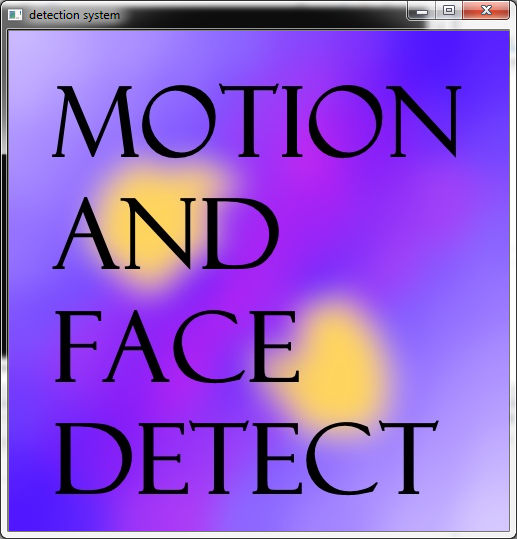
\includegraphics[scale = 0.65]{logo.png}  
  \caption{Окно с логотипом приложения.}
  \label{fig:logo}
\end{figure}

\begin{figure}[ht]
\centering
    \centering
    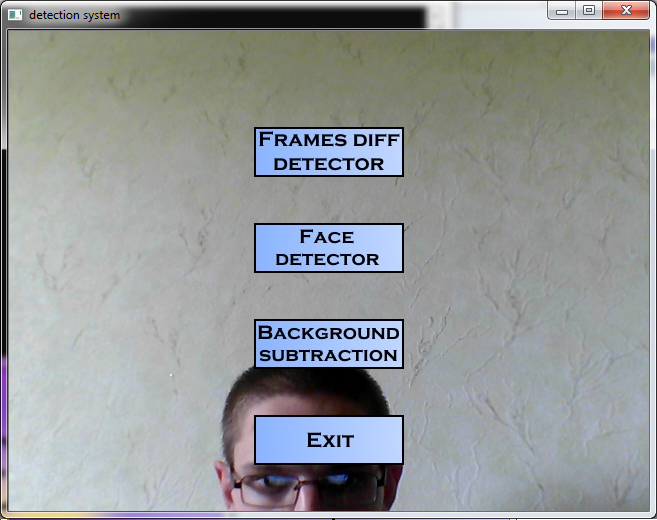
\includegraphics[scale = 0.65]{main_menu.png}  
  \caption{Главное меню.}
  \label{fig:main_menu}
\end{figure}

Пользователь может выбрать любой режим работы приложения, нажав левой кнопкой на соответствующей клавише.
В основном режиме работы приложения(рисунок~\ref{fig:work_mode}) в окне будет две клавиши: сделать снимок изображения или вернуться назад в главное меню.
\begin{figure}[ht]
\centering
    \centering
    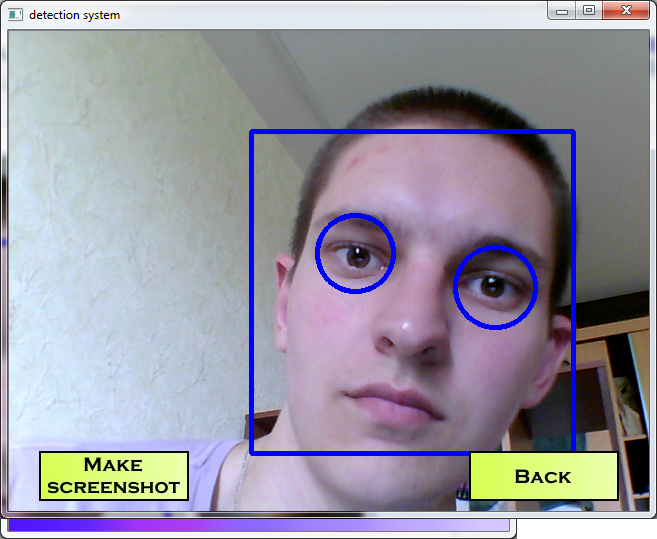
\includegraphics[scale = 0.65]{work_mode.png}  
  \caption{Рабочий режим.}
  \label{fig:work_mode}
\end{figure}

Снимки изображений будут храниться в папке images в каталоге с приложением. В каталоге cascades хранятся входные каскады для обнаружения лица и глаз. Каскады хранятся в формате xml, который используется для хранения данных в OpenCV

